\PassOptionsToPackage{unicode=true}{hyperref} % options for packages loaded elsewhere
\PassOptionsToPackage{hyphens}{url}
%
\documentclass[english,man,floatsintext]{apa7}
\usepackage{lmodern}
\usepackage{amssymb,amsmath}
\usepackage{ifxetex,ifluatex}
\usepackage{fixltx2e} % provides \textsubscript
\ifnum 0\ifxetex 1\fi\ifluatex 1\fi=0 % if pdftex
  \usepackage[T1]{fontenc}
  \usepackage[utf8]{inputenc}
  \usepackage{textcomp} % provides euro and other symbols
\else % if luatex or xelatex
  \usepackage{unicode-math}
  \defaultfontfeatures{Ligatures=TeX,Scale=MatchLowercase}
\fi
% use upquote if available, for straight quotes in verbatim environments
\IfFileExists{upquote.sty}{\usepackage{upquote}}{}
% use microtype if available
\IfFileExists{microtype.sty}{%
\usepackage[]{microtype}
\UseMicrotypeSet[protrusion]{basicmath} % disable protrusion for tt fonts
}{}
\IfFileExists{parskip.sty}{%
\usepackage{parskip}
}{% else
\setlength{\parindent}{0pt}
\setlength{\parskip}{6pt plus 2pt minus 1pt}
}
\usepackage{hyperref}
\hypersetup{
            pdftitle={Modelling disfluencies in copy-typing},
            pdfkeywords={Copy-task; keystroke modelling; autoregression; mixture models; Bayesian statistical models; typing skills},
            pdfborder={0 0 0},
            breaklinks=true}
\urlstyle{same}  % don't use monospace font for urls
\usepackage{graphicx,grffile}
\makeatletter
\def\maxwidth{\ifdim\Gin@nat@width>\linewidth\linewidth\else\Gin@nat@width\fi}
\def\maxheight{\ifdim\Gin@nat@height>\textheight\textheight\else\Gin@nat@height\fi}
\makeatother
% Scale images if necessary, so that they will not overflow the page
% margins by default, and it is still possible to overwrite the defaults
% using explicit options in \includegraphics[width, height, ...]{}
\setkeys{Gin}{width=\maxwidth,height=\maxheight,keepaspectratio}
\setlength{\emergencystretch}{3em}  % prevent overfull lines
\providecommand{\tightlist}{%
  \setlength{\itemsep}{0pt}\setlength{\parskip}{0pt}}
\setcounter{secnumdepth}{0}

% set default figure placement to htbp
\makeatletter
\def\fps@figure{htbp}
\makeatother

% Manuscript styling
\usepackage{upgreek}
\captionsetup{font=singlespacing,justification=justified}

% Table formatting
\usepackage{longtable}
\usepackage{lscape}
% \usepackage[counterclockwise]{rotating}   % Landscape page setup for large tables
\usepackage{multirow}		% Table styling
\usepackage{tabularx}		% Control Column width
\usepackage[flushleft]{threeparttable}	% Allows for three part tables with a specified notes section
\usepackage{threeparttablex}            % Lets threeparttable work with longtable

% Create new environments so endfloat can handle them
% \newenvironment{ltable}
%   {\begin{landscape}\begin{center}\begin{threeparttable}}
%   {\end{threeparttable}\end{center}\end{landscape}}
\newenvironment{lltable}{\begin{landscape}\begin{center}\begin{ThreePartTable}}{\end{ThreePartTable}\end{center}\end{landscape}}

% Enables adjusting longtable caption width to table width
% Solution found at http://golatex.de/longtable-mit-caption-so-breit-wie-die-tabelle-t15767.html
\makeatletter
\newcommand\LastLTentrywidth{1em}
\newlength\longtablewidth
\setlength{\longtablewidth}{1in}
\newcommand{\getlongtablewidth}{\begingroup \ifcsname LT@\roman{LT@tables}\endcsname \global\longtablewidth=0pt \renewcommand{\LT@entry}[2]{\global\advance\longtablewidth by ##2\relax\gdef\LastLTentrywidth{##2}}\@nameuse{LT@\roman{LT@tables}} \fi \endgroup}

% \setlength{\parindent}{0.5in}
% \setlength{\parskip}{0pt plus 0pt minus 0pt}

% \usepackage{etoolbox}
\makeatletter
\patchcmd{\HyOrg@maketitle}
  {\section{\normalfont\normalsize\abstractname}}
  {\section*{\normalfont\normalsize\abstractname}}
  {}{\typeout{Failed to patch abstract.}}
\makeatother
\shorttitle{Modelling disfluencies in copy-typing}
\author{Jens Roeser\textsuperscript{1}, Sven De Maeyer\textsuperscript{2}, Mark Torrance\textsuperscript{1}, Luuk Van Waes\textsuperscript{3}, \& Mariëlle Leijten\textsuperscript{3}}
\affiliation{
\vspace{0.5cm}
\textsuperscript{1} Department of Psychology, Nottingham Trent University, United Kingdom\\\textsuperscript{2} Faculty of Social Sciences, University of Antwerp, Belgium\\\textsuperscript{3} Department of Management, University of Antwerp, Belgium}
\authornote{

Correspondence concerning this article should be addressed to Jens Roeser, 50 Shakespeare St, Nottingham NG1 4FQ. E-mail: jens.roeser@ntu.ac.uk}
\keywords{Copy-task; keystroke modelling; autoregression; mixture models; Bayesian statistical models; typing skills}
\usepackage{csquotes}
\usepackage{booktabs}
\usepackage{longtable}
\usepackage{array}
\usepackage{multirow}
\usepackage{float}
\usepackage{colortbl}
\usepackage{threeparttable}
\usepackage[normalem]{ulem}
\usepackage[utf8]{inputenc}
\ifnum 0\ifxetex 1\fi\ifluatex 1\fi=0 % if pdftex
  \usepackage[shorthands=off,main=english]{babel}
\else
  % load polyglossia as late as possible as it *could* call bidi if RTL lang (e.g. Hebrew or Arabic)
  \usepackage{polyglossia}
  \setmainlanguage[]{english}
\fi

\title{Modelling disfluencies in copy-typing}

\date{}

\abstract{
The analysis of keystroke latency data typically involves the calculation of summary statistics such as the mean inter-keystroke interval, pause frequencies etc. There are two fundamental problems with this: first, descriptives ignore important information in the data and frequently result in biased estimates; second, pauses and pause-related measures are defined using threshold value which are, in principle, arbitrary. We implemented a series of Bayesian models that aimed to address both issues by (a) providing reliable typing estimates and (b) statistically detecting process disfluencies. We tested these models on a random sample of 100 participants from the Dutch copy-task corpus. Our results illustrate how disfluencies can be statistically determined as a mixture of distributions; i.e.~a combination of fluent and disfluent typing intervals characterized by a disfluency magnitude and disfluency probability. Mixture models provide a principled approach to detect disfluencies in keyboard typing data.
}

\begin{document}
\maketitle

\hypertarget{introduction}{%
\section{Introduction}\label{introduction}}

Writing research has made extensive use of keystroke-logging to capture typing process data. In particular process disfluencies (loosely defined as relatively long intervals between subsequent keystrokes) are interesting to develop an understanding of the individuals writing progress. This is because language production is typically thought of as a cascade from the mental generation of a message, into grammatical processing and finally the generation and execution of motor codes that serve the transition of an idea. This can be found in theoretical models of speech (Bock \& Ferreira, 2014), handwriting (Van Galen, 1991) and keyboard typing (Hayes, 2012). Disfluencies at the execution stage are therefore indicators of processing demands that arise on higher levels of mental representation (Christiansen \& Chater, 2016; Olive, 2014); for example, when preplanning syntactic dependencies (Roeser, Torrance, \& Baguley, 2019) or retrieving a lexical entry for a word or its spelling (Torrance, Rønneberg, Johansson, \& Uppstad, 2016). At present there is no principled way of detecting keystroke lags that constitute a process disfluency. In this paper we present a series of statistical models aimed at capturing the typing process and in particular process disfluencies.

Keystroke logs provide rich information about the typing process. From this log, researchers can calculate different process measures including measures of writing fluency (Chukharev-Hudilainen, Saricaoglu, Torrance, \& Feng, 2019; Medimorec \& Risko, 2016; Medimorec, Young, \& Risko, 2017; Van Waes \& Leijten, 2015). To name a few, researchers have performed data analysis on means, medians, standard deviations (SD) etc. of inter-keystroke intervals (the latency between two consecutive keystrokes), number of pauses or pause duration, within-word keystroke intervals and many other variables (for an overview see Conijn et al., 2019a). Conijn et al. (2019a) suggested that these aggregates are sensitive to processing difficulty that arises on different levels of mental representation. However, there are two substantial problems tight to this.

First, researchers made extensive use of pause frequencies, writing bursts and related measures to assess writing performance (e.g. Alves \& Limpo, 2015; Beers, Mickail, Abbott, \& Berninger, 2017; Zhang, Bennett, Deane, \& Rijn, 2019). These measures require a definition of what passes as a pause (Van Waes, Leijten, Lindgren, \& Wengelin, 2016; Wengelin, 2006), i.e.~a pause criterion often set to 2 secs (Chanquoy, Foulin, \& Fayol, 1996; Kaufer, Hayes, \& Flower, 1986; Sullivan \& Lindgren, 2002; Wengelin, 2002) or some other lower bound (Chukharev-Khudilaynen, 2014; Connelly, Dockrell, Walter, \& Critten, 2012; Leijten \& Van Waes, 2013). Researchers have stipulated pause thresholds specific to their research purposes and based on prior research. However, ideally, this threshold would need to be specific to both the writing task and the skills of the typist (Wengelin, 2006). For example, when comparing the frequency of pauses larger than 2 secs for a dyslexic and a normal typist, one might observe more pauses for the dyslexic because 2 secs are indeed not unusual transitions between two keystrokes for a dyslexic writer or pauses for the normal typist are typically shorter than 2 secs and therefore unobserved given the 2 secs pause criterion (Wengelin, 2001). This bias would also affect the interpretation of results from L2 typists and other threshold criteria (Van Waes \& Leijten, 2015).

Second, data aggregation results in the loss of important information about disfluencies and time course variation. Even if this variation is not of interest to answer a research question, parametric aggregates such as the mean and the SD are biased estimates of the typing process. This is because parametric aggregates assume, by definition, that the data must come from a normal distribution for the summary statistic to be representative for the sample. This is not the case as keystroke intervals are zero-bound and therefore right-skewed.\footnote{In fact, the minimum size of keystroke intervals is determined by the time it takes to plan and execute the motor program.} Therefore, data aggregation may lead to incorrect inference based on biased parameter values (Baaijen \& Galbraith, 2018). To prevent biased parameter values, i.e.~to ensure normal distributed data, summary statistics involve data trimming (Hoaglin \& Iglewicz, 1987) to remove data that were \emph{a priori} considered outliers. However, the removal of such disfluencies affects groups of struggling writers more than normal writers and therefore skews the information in the data.

A central methodological challenge with implications for writing research (Hayes, 2012; Kaufer et al., 1986; Van Waes et al., 2016; Wengelin, 2006) is the detection of writing disfluencies. We addressed this problem by implementing statistical models that aim to capture the nature of the data generating process (i.e.~keyboard typing). Crucially we want these models to provide reliable estimates of typing performance without subjecting the data to trimming and threshold criteria, and aggregation.

\hypertarget{modelling-typing-process-data}{%
\section{Modelling typing process data}\label{modelling-typing-process-data}}

As a guiding principle, we aim to produce statistical models that are in line with the mental process that creates the data. The typing process data are measures of the lag between subsequent keypresses, for example, the transitions c\(^{\wedge}\)a\(^{\wedge}\)t for the word \emph{cat} where \(^{\wedge}\) respectively indicates the inter-keystroke interval (IKI) between pressing \(<\)c\(>\) and \(<\)a\(>\), and \(<\)a\(>\) and \(<\)t\(>\). Further, our models should provide a systematic way of addressing process disfluencies; when the lag before pressing \(<\)a\(>\) is unusually large. We implemented a series of possible models for the keystroke data. The quality of these models will be compared in the Results section.

Statistical models can be used to characterize an underlying data generating process as a function with parameter values. For example, if we assume that the process of interest can be described as normal distribution, we need a mean \(\mu\) and a variance \(\sigma^2\) to draw this distribution. The values of the parameters \(\mu\) and \(\sigma^2\) are unknown and often expected to vary across task demands and population. This model can be written as \(y \sim Normal(\mu, \sigma^2)\); the data \(y\) come from a process that follows a normal distribution with an unknown mean \(\mu\) and an unknown error variance \(\sigma^2\). Our statistical models need to determine values for these parameters that can be considered reliable. Bayesian models, as used in this paper, are ideal for reliable parameter estimation as they allow us to derive a probability distribution of the parameter value of interest (Farrell \& Lewandowsky, 2018; Gelman et al., 2014; Lee \& Wagenmakers, 2014). To achieve this, Bayesian models require the explicit inclusion of prior information, i.e.~existing knowledge about parameter values. For small data sets even vague priors influences the posterior (inferred parameter estimates) but for larger data sets the posterior is overcome by the data (i.e.~automatic Ockam's razor; Jefferys \& Berger, 1992). In the present papar, priors are used to aid model convergence by constraining the parameter space (i.e.~using weakly regulating priors; Lambert, 2018; McElreath, 2016).

We assume throughout that IKIs can be characterized as log-normal distributed because IKIs are zero-bound (Baayen, 2008). To be able to estimate the parameter of interest, the mean \(\mu\), we need a model that accounts for other sources of variance. This can easily be achieved with linear mixed effects models (LMM) which has been used to model keystroke data (Leijten, De Maeyer, \& Van Waes, 2011; Quené \& Van den Bergh, 2004; Van Waes, Leijten, \& Quinlan, 2010; Van Waes, Leijten, Roeser, Olive, \& Grabowski, 2020). The LMM in equation \ref{eq:lmm} is an extension of the simple example above. Sources of random error variance in this model are participants \(u\) and bigrams \(w\).

\[
\tag{1}
\begin{aligned}
y_{ij} \sim LogNormal(\mu + u_i + w_j, \sigma_e^2)\\
\end{aligned}
\label{eq:lmm}
\]

In particular, some participants are faster typists than others. These differences associated with participant \(i\), expressed as \(u_i\), can be assumed to be normal distributed around 0 with a between participants variance \(\sigma_u^2\) with \(i = 1, \dots, I\), where \(I\) is the number of participants (see \ref{eq:lmm2}). The variance \(\sigma_u^2\) is given a half-Normal prior with a mean of 0 and a variance of 2.5.

\[
\tag{2}
\begin{aligned}
u_i \sim Normal(0,\sigma_u^2)\\
\sigma_u \sim Normal(0,2.5)\\
\text{constraint: } \sigma_u >0 
\end{aligned}
\label{eq:lmm2}
\]

Variation between keystroke pairs (i.e.~letter bigrams) \(w\) is added as random intercepts term in equation \ref{eq:lmm} (Van Waes, Leijten, Pauwaert, \& Van Horenbeeck, 2019; Van Waes et al., 2020). More specifically, this it to assume that each bigram \(j\) with \(j = 1, \dots, J\), where \(J\) is the total number of bigrams, is independent of the other bigrams. Each bigram intercept difference \(w_j\) is distributed around 0 with a between bigram variance \(\sigma_w^2\) (equation \ref{eq:lmm5}).

\[
\tag{3}
\begin{aligned}
w_j \sim Normal(0,\sigma_w^2)\\
\sigma_w \sim Normal(0,2.5)\\
\text{constraint: }\sigma_w >0 
\end{aligned}
\label{eq:lmm5}
\]

In other words, the parameter estimate for the mean \(\mu\) in equation \ref{eq:lmm} is the marginalised values after taking into account random variation between participants \(u\) and bigrams \(w\). To aid effective sampling, we non-centred the mean \(\mu\) in all models with regulating priors (equation \ref{eq:lmm3}; see Lambert, 2018).

\[
\tag{4}
\begin{aligned}
\mu = \alpha_{\mu} + \sigma_{\mu} * \mu_{\text{raw}}\\
\alpha_{\mu} \sim Normal(5,2)\\
\sigma_{\mu} \sim Normal(0,10)\\
\mu_{\text{raw}} \sim Normal(0,1)\\
\text{constraint: }\mu_{\sigma}>0 
\end{aligned}
\label{eq:lmm3}
\]

For the unexplained variance \(\sigma_e^2\) we used an uninformative half-Cauchy prior (equation \ref{eq:lmm4}; see Gelman et al., 2014).

\[
\tag{5}
\begin{aligned}
\sigma_e \sim Cauchy(0,2.5)\\
\text{constraint: }\sigma_e>0 
\end{aligned}
\label{eq:lmm4}
\]

Further, we can extend this model by assuming that larger variations in typing differences for bigrams depend on the typing speed of each participant. For example, fast participants might show less variation between bigrams than slow participants. This assumption can be modelled by including by-participant slope adjustments for bigrams by introducing a variance-covariance matrix \(\Sigma_u\); LKJ prior with \(\nu=2.0\) (Lewandowski, Kurowicka, \& Joe, 2009).

\hypertarget{typing-as-autoregressive-process}{%
\subsection{Typing as autoregressive process}\label{typing-as-autoregressive-process}}

The previous model captures variation associated with particular bigrams but assumes that disfluencies are subject to random noise. Further, the standard analysis assumes that subsequent keystrokes are independent and thus exchangeable. IKIs are not necessarily independent; IKI\(_{i}\) might be related to IKI\(_{i-1}\) preceding it (Conijn et al., 2019b). In other words, we can predict an IKI with the previous keystroke and capture their relationship with a parameter \(\phi\); see equation \ref{eq:ark}. This is called an autoregressive process (Eltahir, Salami, Ismail, \& Lai, 2004). This model captures disfluencies as slowdown relative to a previous keystroke. The autocorrelation was assumed to vary for each participant \(\phi_i\) with a centred mean \(\mu_{\phi}\) and error variance \(\eta^2\).

\[
\tag{6}
\begin{aligned}
y_{ij} \sim LogNormal(\mu + \phi_i*log(y_{ij-1}) + u_i, \sigma_e^2)\\
\text{where}\\
\phi_i \sim Normal(\mu_{\phi}, \eta^2)\\
\mu_{\phi} \sim Normal(0, 1)\\
\eta \sim Cauchy(0, 1)\\
\text{constraint: }\eta >0 
\end{aligned}
\label{eq:ark}
\]

\hypertarget{typing-as-mixture-process}{%
\subsection{Typing as mixture process}\label{typing-as-mixture-process}}

Disfluencies can also be captured in finite mixture models. Mixture models assume that data come from a combination of distributions. For the present purpose we constrain the model to be finite. In other words, we fixed the number of underlying distributions to two, namely 2 log-Gaussian (normal) distributions, of which one represents fluent typing (shorter IKIs) and the other represents disfluencies (longer IKIs). This model can be summarised as in equation \ref{eq:mog}, following Vasishth, Chopin, Ryder, and Nicenboim (2017). The first and second line are the sum of two log-normal distributions of which the first distribution has a mixing proportion (weight) \(\theta\) and the other distribution receives the remaining proportion \(1-\theta\). Both distributions have the same mean \(\mu\) but the parameter \(\delta\) that added to the first distribution and constrained to be positive. Thus, \(\delta\) captures the magnitude of the disfluency. The mixing proportion \(\theta_i\), then, captures the probability of disfluent IKIs for each participant \(i\).

\[
\tag{7}
\begin{aligned}
    y_{ij} \sim \theta_i \cdot LogNormal(\mu + \delta + u_i + w_j, \sigma_{e'}^2) +\\
        (1 - \theta_i) \cdot LogNormal(\mu + u_i + w_j, \sigma_{e}^2)\\
        \text{where}\\
        \delta \sim Normal(0,1)\\
        \text{constraint: } \delta > 0
\end{aligned}   
\label{eq:mog}
\]

The hyper-parameter \(\mu_{\theta}\) captures the population disfluency probability (with an error variance \(\tau^2\)) as shown in equation \ref{eq:mog2}. The mixing proportion \(\theta_i\) was transformed to range from 0 to 1 (inverse logit) where a value of 0 would indicate fluent typing and 1 indicates disfluency.

\[
\tag{8}
\begin{aligned}
        \theta_i = Logit^{-1}(\theta_i)\\
        \theta_i \sim Normal(\mu_{\theta},\tau^2)\\
        \mu_{\theta} \sim Normal(0,1)\\
        \tau \sim Cauchy(0,1)\\
        \text{constraint: } \tau > 0
\end{aligned}   
\label{eq:mog2}
\]

As longer latencies are known to be associated with a larger variances for both response-time data in particular (Wagenmakers \& Brown, 2007) and human motor behaviour in general (Schöner, 2002; Wing \& Kristofferson, 1973), the variance \(\sigma_{e'}^2\) associated with the distribution of typing disfluencies was constrained to be larger than the variance for normal typing \(\sigma_e^2\) as shown in \ref{eq:mog3} (see Vasishth et al., 2017; Vasishth, Jäger, \& Nicenboim, 2017).

\[
\tag{9}
\begin{aligned}
        \sigma_{e'} = \sigma + \sigma_{\text{diff}}\\
        \sigma_{e} = \sigma - \sigma_{\text{diff}}\\
        \sigma_{\text{diff}} \sim Normal(0,1)\\
        \sigma \sim Cauchy(0,2.5)\\
        \text{constraint: } \sigma, \sigma_{\text{diff}}, \sigma_{e'}, \sigma_{e} > 0
\end{aligned}   
\label{eq:mog3}
\]

\hypertarget{typing-as-autoregressive-mixture-process}{%
\subsection{Typing as autoregressive mixture process}\label{typing-as-autoregressive-mixture-process}}

Note that the mixture model, as well as the LMM, implies that subsequent keystroke intervals are independent. This might be the case for disfluencies but subsequent IKIs in fluent typing might involve autocorrelations. Therefore, we implemented another mixture model but replaced the bigram intercepts \(w_j\), in the distribution that represents fluent typing in equation \ref{eq:mog}, with an autoregressor \(\phi_i*y_{ij-1}\), as in equation \ref{eq:ark}; random bigram intercepts were kept for the distribution of disfluent typing intervals.

\hypertarget{method}{%
\section{Method}\label{method}}

To test which model captures the typing process best, we applied a series of models as described in the previous section to data from a subset of the Dutch copy-task corpus (Leijten \& Van Waes, 2013; Van Waes et al., 2019; Van Waes et al., 2020). An overview of all models can be found in Table \ref{tab:models}.

\begin{table}[!ht]

\begin{center}
\begin{threeparttable}

\caption{\label{tab:models}Overview of typing process models. All models were fitted with random intercepts for participants.}

\begin{tabular}{llll}
\toprule
Models & \multicolumn{1}{c}{Type} & \multicolumn{1}{c}{Equation} & \multicolumn{1}{c}{Description}\\
\midrule
M1 & LMM & \ref{eq:lmm} & Random intercepts for bigram order\\
M2 & LMM &  & As M1; by-participant random bigram slopes\\
M3 & AR & \ref{eq:ark} & Autocorrelation between subsequent IKIs\\
M4 & MoG & \ref{eq:mog} & Mixture process of normal and disfluent typing\\
M5 & AR + MoG &  & As M4 but autocorrelation for normal typing\\
\bottomrule
\addlinespace
\end{tabular}

\begin{tablenotes}[para]
\normalsize{\textit{Note.} LMM = Linear mixed effects models; AR = Autoregressive model; MoG = Mixture of (log-)Gaussians}
\end{tablenotes}

\end{threeparttable}
\end{center}

\end{table}

The copy-task corpus consists of keystroke data collected in Inputlog, a Javascript-based web application available on \url{www.inputlog.net} with the source released on \url{https://github.com/lvanwaes/Inputlog-Copy-Task} and \url{https://zenodo.org/record/2908966}. In a set of different subtasks participants have to produce keyboard typed responses (a sentence, various phrases and consonants). In this analysis we focus on the consonant task. Participants saw and copy-typed a single time four blocks of six consonant sequences \enquote{tjxgfl pgkfkq dtdrgt npwdvf}. This task allows us to measure typing skills in a non-linguistic environment (Grabowski, Weinzierl, \& Schmitt, 2010). Importantly for the present purpose, fluent copying and pausing is a function of the participant's memory span and typing skill such that touch-typists depend less on holding sequences in memory for fluent copying than hunt-and-peck typists. This results in a combination of fluent typing and typing interruptions. In other words, for this task we need to be able to disentangle fluent and disfluent IKIs. We used a random sample of 100 participants (78 females, 22 males) from the age range of 18 to 25 years (median age = 22 years). Before analysis we excluded spaces and editing operations from the data. To allow comparisons between the autoregressive model and all other models we had exclude the first IKI for each participant.

\hypertarget{results}{%
\section{Results}\label{results}}

\hypertarget{data-overview}{%
\subsection{Data overview}\label{data-overview}}

The raw data are visualized in Figure \ref{fig:descriptives}. In the upper panel of Figure \ref{fig:descriptives}A each line represents one participant. In the lower panel of Figure \ref{fig:descriptives}A the coloured lines show different measures of central tendency which are also shown in the density plot in Figure \ref{fig:descriptives}B. This figure highlights: (1) aggregating data ignores individual disfluencies patterns in the data; (2) the choice of central tendency measure might lead to different conclusions about patterns in the data. Figure \ref{fig:descriptives}A shows that participants slow down and speed up for some but not the same bigrams. The figure suggests that this is not a learning effect or a tendency to fatique. Central tendency measures in the lower panel of Figure \ref{fig:descriptives}A suggest that some slowdowns might be bigram specific (e.g. \(<\)jx\(>\), \(<\)td\(>\)). Importantly though, this graph suggests that the choice of central tendency measure might affect whether we consider an observation a disfluency. For example, a slowdown from \(<\)pg\(>\) to \(<\)gk\(>\) median and mean, but not the mode, suggest a disfluency. Similarily a speedup tendency can be observed in mean and median but not in the mode from \(<\)gk\(>\) to \(<\)kf\(>\). Figure \ref{fig:descriptives}B shows why this might be the case. Shown is the density distribution of the IKI data. The distribution is skewed (although log-scaled) with a bimodal tendency. While mean, median and mode are the same for a normal distribution, they are representing different properties of a non-normal sample distribution. In particular, means are known to be more sensitive to long values which are inevitible as IKIs are zero-bound (cannot be smaller than zero) but have, in principle, no upper bound. In other words, means are closer to the horizontal middle of the distribution which, for right-skewed distributions, is on the right of the peak of the distribution (of observations with the highest kernel density). The latter is being represented by the mode. The median appears to be a sensible compromise as it is less supceptive to extreme values than the mean. However, all three central tendencies are problematic as they ignore important property of the distribution, i.e.~the combination of regular and slow IKIs. In other words, data aggregation may hide participant-specific disfluencies and some patterns observed in the data may depend on the choice of central tendency.

\begin{figure}[!ht]

{\centering 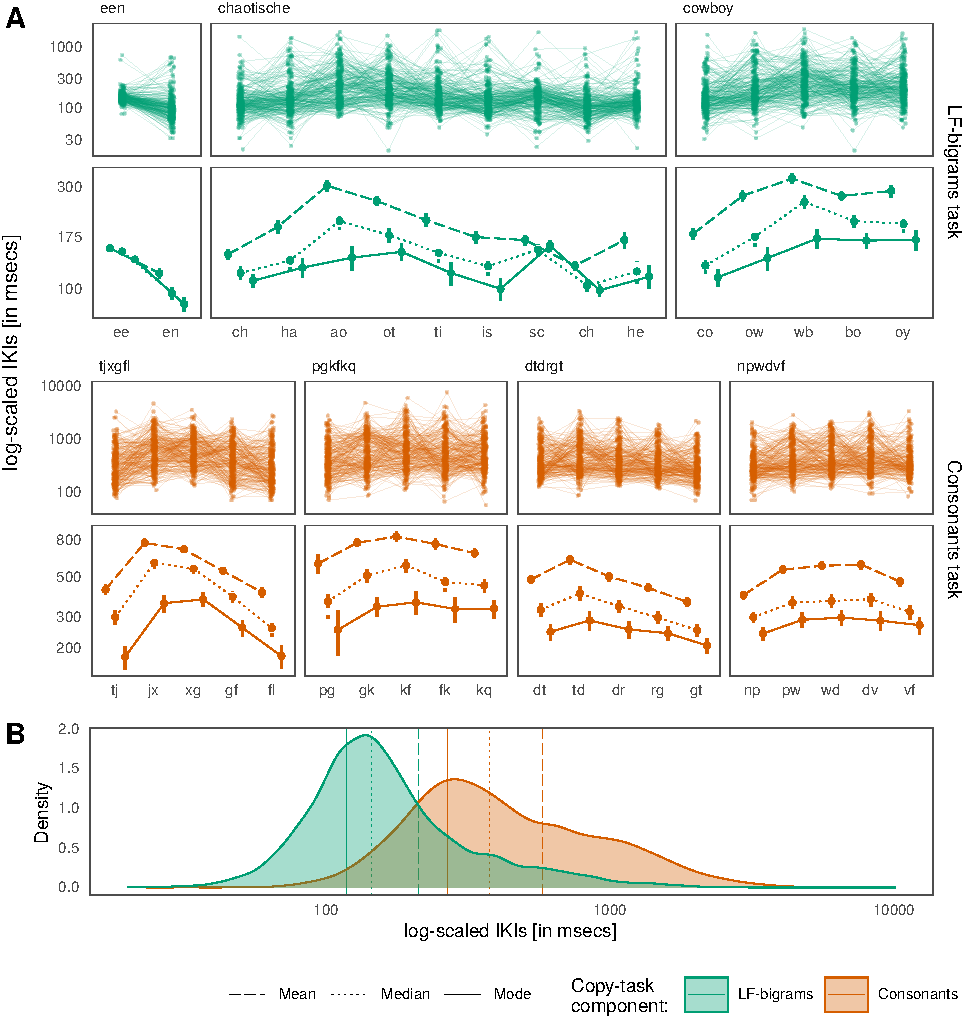
\includegraphics{report_files/figure-latex/descriptives-1} 

}

\caption{Descriptive summary of IKI data. Panel A illustrates IKI over bigrams position (time course) by participant in the upper row and as different measures of central tendency in the middle row (with standard error [SE]). Panel B shows the density distribution of IKI data with the same central tendency descriptors as in panel A.}\label{fig:descriptives}
\end{figure}

\hypertarget{model-fit}{%
\subsection{Model fit}\label{model-fit}}

All models were implemented as Bayesian models (see e.g. Gelman et al., 2014; Lambert, 2018; McElreath, 2016) in the probabilistic programming language Stan (Carpenter et al., 2016; Hoffman \& Gelman, 2014; Stan Development Team, 2015a, 2015b). \textit{R} and \textit{Stan} code are available on GitHub (\href{https://github.com/jensroes/Typing-disfluency}{github.com/jensroes/Typing-disfluency}). Models were fitted with 30,000 iterations (15,000 warm-up) on 3 MCMC chains. Convergence was tested via the Rubin-Gelman statistic (Gelman \& Rubin, 1992), traceplots and cross-validation (Vehtari, Gelman, \& Gabry, 2015, 2017).

The predictive performance of the models was established using leave-one-out cross-validation. Cross-validation penalizes models with more parameters and therefore prevents overfit (see Farrell \& Lewandowsky, 2018; Lambert, 2018; Lee \& Wagenmakers, 2014; McElreath, 2016). The out-of-sample predictive performance was determined via Pareto smoothed importance-sampling (Vehtari et al., 2015, 2017) and estimated as sum of the expected log predictive density (\(\widehat{elpd}\)). \(\widehat{elpd}\) was used to compare the predictive quality of our models. Model comparisons can be found in Table \ref{tab:modelcomparisons}. The mixture model M4 (see equation \ref{eq:mog}) revealed the highest predictive performance.

\begin{table}[!ht]

\begin{center}
\begin{threeparttable}

\caption{\label{tab:modelcomparisons}Model comparisons expressed as expected log predictive density ($\widehat{elpd}$). The top row shows the model with the highest predictive performance. Differences in predictive performance are shown as $\Delta\widehat{elpd}$. Standard errors (SE) are shown in brackets.}

\begin{tabular}{llrr}
\toprule
Model & \multicolumn{1}{c}{Type} & \multicolumn{1}{c}{$\Delta\widehat{elpd}$} & \multicolumn{1}{c}{$\widehat{elpd}$}\\
\midrule
M4 & MoG & 0 (0) & -13857 (59)\\
M5 & AR + MoG & -14 (14) & -13871 (57)\\
M2 & LMM & -87 (24) & -13944 (53)\\
M1 & LMM & -153 (18) & -14010 (54)\\
M3 & AR & -223 (21) & -14080 (54)\\
\bottomrule
\addlinespace
\end{tabular}

\begin{tablenotes}[para]
\normalsize{\textit{Note.} LMM = linear mixed effects models; AR = Autoregressive model; MoG = Mixture of (log-)Gaussians}
\end{tablenotes}

\end{threeparttable}
\end{center}

\end{table}

The second best performing model is the mixture model with the autoregressor \(phi\) for fluent typing. In other words, adding the autoregressor instead of random bigram intercepts for fluent typing did not improve the predictive performance of the model. In fact, the autoregressive model was found to be the model with the lowest predictive performance. Modelling bigrams as random intercepts (with and without by-participant slope adjustments) was found to have a higher predictive performance compared to the autoregession model.

\hypertarget{parameter-evaluation}{%
\subsection{Parameter evaluation}\label{parameter-evaluation}}

The copy-typing process captured by the mixture model can be characterized with the posterior distributions of the model's parameter values. The process relevant parameters are illustrated in Figure \ref{fig:parameters}. Firstly, IKIs, excluding disfluencies, are shown by participant in Figure \ref{fig:parameters}A. The red line indicates the pooled overall parameter estimate for fluent typing, i.e. \(\hat{\beta}\)=259 msecs centred around a 95\% PI of {[}235, 286{]}. For each participant the probability of disfluent typing is shown in Figure \ref{fig:parameters}B. The overall disfluency probability (in red) was \(\hat{\theta}\)=0.73 centred around 95\% PI{[}0.63, 0.83{]}. In other words, for the consonant task we observe 73\% disfluent typing and 27\% fluent typing.

The y-axis in panel A and B are ordered by the average size of the respective values, thus the lines do not represent the same participants. In fact, Figure \ref{fig:parameters}C suggests that the inferred latency for fluent typing and the probability to exhibit disfluencies are independent. Shown are the parameter estimates for each participant and the overall pooled estimates. In other words, fast as well as slow copy-typists can show low and high disfluency probabilities. Finally, the slowdown for disfluent typing is shown in Figure \ref{fig:parameters}D. Disfluent typing in the consonant task is \(\hat{\delta}\)=297 msecs (95\% PI{[}251, 347{]}) slower than fluent.\footnote{Faster participants might show larger disfluencies magnitudes; i.e.~the size of the disfluency \(\delta\) may vary by participant. This was not supported for the consonant copy-task. Allowing \(\delta\) to vary by participant renders a negligible gain over model M4 (\(\Delta\widehat{elpd}\)=3, SE=2); holding \(\theta\) constant while allowing \(\delta\) to vary by participant revealed a lower predictive performance (\(\Delta\widehat{elpd}\)=-48, SE=14).} Overall, for these data it is crucial to distinguish between fluent and disfluent typing. This is because disfluencies are indeed more common than fluent transitions in this task. Not distinguishing between fluent and disfluent typing would lead to the incorrect inference that the task complexity affects the keystroke transitions throughout while this is not true for roughly one-third of the data. Mixture models can provide accurate estimates for fluent typing while account for disfluencies by modelling fluent and disfluent typing as a mixture process.

\begin{figure}[!ht]

{\centering 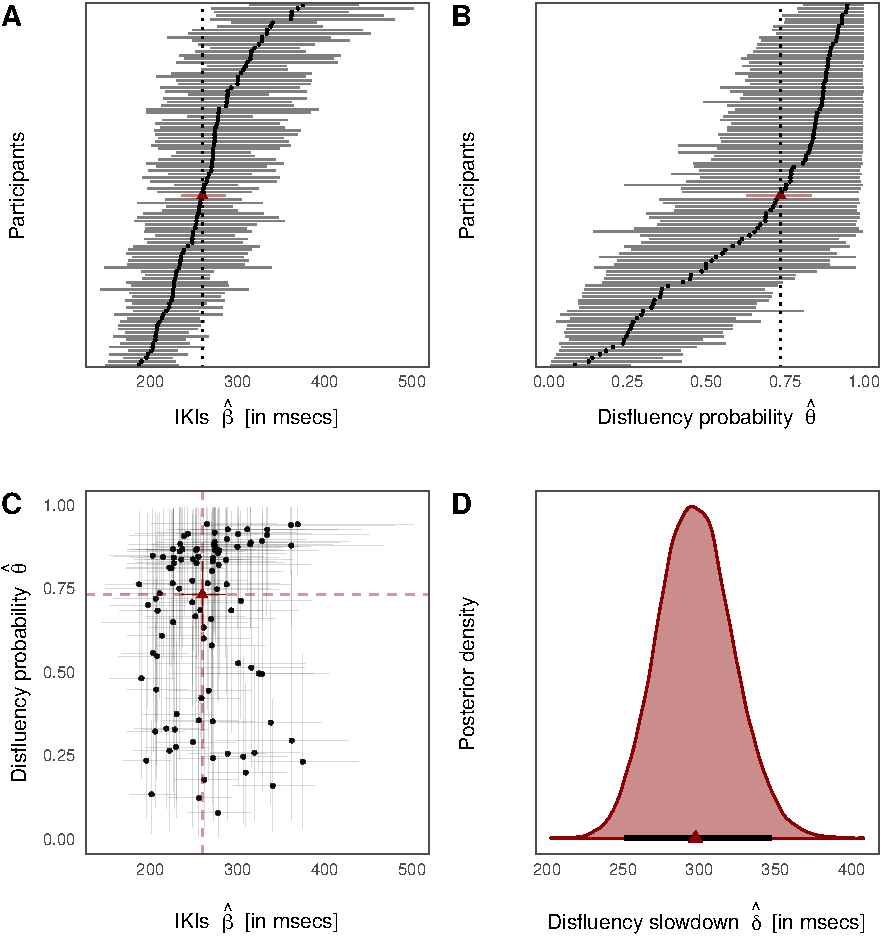
\includegraphics{report_files/figure-latex/parameters-1} 

}

\caption{Posterior parameter values of the mixture model. Panel A shows by-participant IKIs and overall IKI value for fluent typing in red. Panel B shows by-participant disfluency probability (overall parameter value $\theta$ in red). Panel C shows fluent IKIs plotted against disfluency probability (red triangle indicates overall parameter value). Panel D shows the posterior distribution of the disfluency slowdown. All error bars are 95\% probability intervals.}\label{fig:parameters}
\end{figure}

\hypertarget{discussion}{%
\section{Discussion}\label{discussion}}

Our aim was to provide a statistical model of inter-keystroke intervals that addresses process disfluencies in a principled manner. We compared a series of Bayesian models addressing this aim. Model comparisons showed that process disfluencies can be captured as a mixture process for the consonant copy-task. This model allows us to extract reliable typing-interval estimates for fluent typing while accounting for process disfluencies by modelling fluent and disfluent typing as a combination of two distributions with a latent mixing ratio.

This model provides a probability distribution of the parameter values for a) fluent typing, overall and by-participant, b) the disfluency probability, overall and by-participant, and c) the disfluency magnitude (i.e.~typing slowdown). These parameter estimates are relevant on two levels. First, they allow us to characterize the writing task at hand. For example, we observed that copy-typing non-lexical strings of consonants shows indeed a larger proportion of disfluent compared to fluent typing. Second, by-participant parameter estimates allow us to extract typing characteristics for individual typists. In particular, we extracted each participants' fluent typing speed and the probability of disfluencies exhibited by each participant. This disfluency probability for the consonant task can be understood as an indicator of memory span (Grabowski et al., 2010; Olive, 2014) and low level reading skill (De Smet, Leijten, \& Van Waes, 2018) and depends on individual typing skills. If participants with a smaller memory span look more often to the target string, they will show a larger proportion of typing disfluencies. Taken together with the overall and individual parameter estimates, we can determine whether an individual was a fast / slow typist or had unusually high / low probability to exhibit disfluencies compared to the population estimates. Thus, the model can be used diagnostically to identify participants with larger disfluency probabilities or to compare pausing across groups of participants.

The central advantage of using mixture models to account for typing disfluencies is that we can by-pass the use of threshold values to define disfluencies and include it as individual typing skill characteristic in the analysis of writing process data. From the raw data it is not possible to know which data are disfluencies. Using threshold values ignores that some participants are generally slower typists and some tasks are more difficult. Mixture models allow us to capture disfluencies as a latent process in a principled way. This is important because our mixture models take into account that a disfluency is relative to an individuals' typing speed and the task at hand (Wengelin, 2006). Therefore, these models allow us to test predictions about typing disfluencies in certain population such as learning typists, L2 typists and individuals with genuine typing difficulty after account for individual differences in typing speed or vice versa. In other words, the presented model can be used to test hypothesis about psychological factors (e.g.~memory demands, writing experience, proficiency in writing in a second language) that might affect the ratio of disfluencies in the writing process. If disfluencies are crutial to identify certain individuals in a sample, this mixture model might also be used as diagnostic tool. As an avenue for future research, mixture models as presented in this paper can be used for different types of writing tasks and particular populations.

Writing involves processing on various levels of mental representation. As activation cascades from higher to lower levels of representation, a delay on any of these levels causes disfluencies. While we distinguished fluent and disfluent typing in a binary way, processing difficulty on different levels might be associated with different disfluency magnitudes and might be cumulative. If the size of the disfluency is assumed to depend on the inhibited process upstream or combination of processes, this can be implemented as additional mixture component(s) (similar to Baaijen, Galbraith, \& de Glopper, 2012) to address different types of disfluencies (Medimorec \& Risko, 2016; Medimorec et al., 2017; Wengelin, 2001). In other words extensions of mixture models allow us to test different hypotheses about the cascade of processes involved in writing and language production.

\hypertarget{references}{%
\section{References}\label{references}}

\begingroup
\setlength{\parindent}{-0.5in}
\setlength{\leftskip}{0.5in}

\hypertarget{ref}{}

\endgroup

\hypertarget{refs}{}
\leavevmode\hypertarget{ref-alves2015progress}{}%
Alves, R. A., \& Limpo, T. (2015). Progress in written language bursts, pauses, transcription, and written composition across schooling. \emph{Scientific Studies of Reading}, \emph{19}(5), 374--391.

\leavevmode\hypertarget{ref-baaijen2018discovery}{}%
Baaijen, V. M., \& Galbraith, D. (2018). Discovery through writing: Relationships with writing processes and text quality. \emph{Cognition and Instruction}, \emph{36}(3), 199--223.

\leavevmode\hypertarget{ref-baaijen2012keystroke}{}%
Baaijen, V. M., Galbraith, D., \& de Glopper, K. (2012). Keystroke analysis: Reflections on procedures and measures. \emph{Written Communication}, \emph{29}(3), 246--277.

\leavevmode\hypertarget{ref-baa08book}{}%
Baayen, R. H. (2008). \emph{Analyzing linguistic data. A practical introduction to statistics using R}. Cambridge: Cambridge University Press.

\leavevmode\hypertarget{ref-beers2017effects}{}%
Beers, S. F., Mickail, T., Abbott, R., \& Berninger, V. (2017). Effects of transcription ability and transcription mode on translation: Evidence from written compositions, language bursts and pauses when students in grades 4 to 9, with and without persisting dyslexia or dysgraphia, compose by pen or by keyboard. \emph{Journal of Writing Research}, \emph{9}(1), 1--25.

\leavevmode\hypertarget{ref-bock2014syntactically}{}%
Bock, J. K., \& Ferreira, V. S. (2014). Syntactically speaking. In M. Goldrick, V. S. Ferreira, \& M. Miozzo (Eds.), \emph{The Oxford Handbook of Language Production} (pp. 21--46). Oxford: Oxford University Press.

\leavevmode\hypertarget{ref-carpenter2016stan}{}%
Carpenter, B., Gelman, A., Hoffman, M. D., Lee, D., Goodrich, B., Betancourt, M., \ldots{} Riddell, A. (2016). Stan: A probabilistic programming language. \emph{Journal of Statistical Software}, \emph{20}.

\leavevmode\hypertarget{ref-chanquoy1996writing}{}%
Chanquoy, L., Foulin, J.-N., \& Fayol, M. (1996). Writing in adults: A real-time approach. In G. Rijlaarsdam, H. Van den Bergh, \& M. Couzijn (Eds.), \emph{Theories, models and methodology in writing research} (pp. 36--44). Amsterdam: Amsterdam University Press.

\leavevmode\hypertarget{ref-christiansen2016now}{}%
Christiansen, M. H., \& Chater, N. (2016). The now-or-never bottleneck: A fundamental constraint on language. \emph{Behavioral and Brain Sciences}, \emph{39}, 1--72. \href{https://doi.org/\%20http://dx.doi.org/10.1017/S0140525X1500031X}{https://doi.org/ http://dx.doi.org/10.1017/S0140525X1500031X}

\leavevmode\hypertarget{ref-chukharev2019combined}{}%
Chukharev-Hudilainen, E., Saricaoglu, A., Torrance, M., \& Feng, H.-H. (2019). Combined deployable keystroke logging and eyetracking for investigating L2 writing fluency. \emph{Studies in Second Language Acquisition}, \emph{41}(3), 583--604.

\leavevmode\hypertarget{ref-chukharev2014pauses}{}%
Chukharev-Khudilaynen, E. (2014). Pauses in spontaneous written communication: A keystroke logging study. \emph{Journal of Writing Research}, \emph{6}(1), 61--84.

\leavevmode\hypertarget{ref-conijn2019understanding}{}%
Conijn, R., Roeser, J., \& van Zaanen, M. (2019a). Understanding the keystroke log: The effect of writing task on keystroke features. \emph{Reading and Writing}, \emph{32}(9), 2353--2374.

\leavevmode\hypertarget{ref-conijn2019typo}{}%
Conijn, R., Van Zaanen, M., Leijten, M., \& Van Waes, L. (2019b). How to typo? Building a process-based model of typographic error revisions. \emph{The Journal of Writing Analytics}, \emph{3}, 69--95.

\leavevmode\hypertarget{ref-connelly2012predicting}{}%
Connelly, V., Dockrell, J. E., Walter, K., \& Critten, S. (2012). Predicting the quality of composition and written language bursts from oral language, spelling, and handwriting skills in children with and without specific language impairment. \emph{Written Communication}, \emph{29}(3), 278--302.

\leavevmode\hypertarget{ref-de2018exploring}{}%
De Smet, M. J. R., Leijten, M., \& Van Waes, L. (2018). Exploring the process of reading during writing using eye tracking and keystroke logging. \emph{Written Communication}, \emph{35}(4), 411--447.

\leavevmode\hypertarget{ref-eltahir2004dynamic}{}%
Eltahir, W. E., Salami, M., Ismail, A. F., \& Lai, W. (2004). Dynamic keystroke analysis using AR model. In \emph{IEEE international conference on industrial technology} (Vol. 3, pp. 1555--1560). IEEE.

\leavevmode\hypertarget{ref-farrell2018computational}{}%
Farrell, S., \& Lewandowsky, S. (2018). \emph{Computational modeling of cognition and behavior}. Cambridge University Press.

\leavevmode\hypertarget{ref-gelman2014}{}%
Gelman, A., Carlin, J. B., Stern, H. S., Dunson, D. B., Vehtari, A., \& Rubin, D. B. (2014). \emph{Bayesian data analysis} (3rd ed.). Chapman; Hall/CRC.

\leavevmode\hypertarget{ref-gelman1992}{}%
Gelman, A., \& Rubin, D. B. (1992). Inference from iterative simulation using multiple sequences. \emph{Statistical Science}, \emph{7}(4), 457--472.

\leavevmode\hypertarget{ref-grabowski2010second}{}%
Grabowski, J., Weinzierl, C., \& Schmitt, M. (2010). Second and fourth graders' copying ability: From graphical to linguistic processing. \emph{Journal of Research in Reading}, \emph{33}(1), 39--53.

\leavevmode\hypertarget{ref-hayes2012evidence}{}%
Hayes, J. R. (2012). Evidence from language bursts, revision, and transcription for translation and its relation to other writing processes. In M. Fayol, D. Alamargot, \& V. Berninger (Eds.), \emph{Translation of thought to written text while composing} (pp. 15--25). New York, NY: Psychology Press.

\leavevmode\hypertarget{ref-hoaglin1987fine}{}%
Hoaglin, D. C., \& Iglewicz, B. (1987). Fine-tuning some resistant rules for outlier labeling. \emph{Journal of the American Statistical Association}, \emph{82}(400), 1147--1149.

\leavevmode\hypertarget{ref-hoffman2014no}{}%
Hoffman, M. D., \& Gelman, A. (2014). The No-U-Turn sampler: Adaptively setting path lengths in Hamiltonian Monte Carlo. \emph{Journal of Machine Learning Research}, \emph{15}(1), 1593--1623.

\leavevmode\hypertarget{ref-jefferys1992ockham}{}%
Jefferys, W. H., \& Berger, J. O. (1992). Ockham's razor and Bayesian analysis. \emph{American Scientist}, \emph{80}(1), 64--72.

\leavevmode\hypertarget{ref-kaufer1986composing}{}%
Kaufer, D. S., Hayes, J. R., \& Flower, L. (1986). Composing written sentences. \emph{Research in the Teaching of English}, \emph{20}(2), 121--140.

\leavevmode\hypertarget{ref-lambert2018student}{}%
Lambert, B. (2018). \emph{A student's guide to Bayesian statistics}. Sage.

\leavevmode\hypertarget{ref-lee2014bayesian}{}%
Lee, M. D., \& Wagenmakers, E.-J. (2014). \emph{Bayesian cognitive modeling: A practical course}. Cambridge University Press.

\leavevmode\hypertarget{ref-leijten2011coordinating}{}%
Leijten, M., De Maeyer, S., \& Van Waes, L. (2011). Coordinating sentence composition with error correction: A multilevel analysis. \emph{Journal of Writing Research}, \emph{2}(3), 331--363.

\leavevmode\hypertarget{ref-leijten2013keystroke}{}%
Leijten, M., \& Van Waes, L. (2013). Keystroke logging in writing research: Using Inputlog to analyze and visualize writing processes. \emph{Written Communication}, \emph{30}(3), 358--392.

\leavevmode\hypertarget{ref-lewandowski2009generating}{}%
Lewandowski, D., Kurowicka, D., \& Joe, H. (2009). Generating random correlation matrices based on vines and extended onion method. \emph{Journal of Multivariate Analysis}, \emph{100}(9), 1989--2001.

\leavevmode\hypertarget{ref-mcelreath2016statistical}{}%
McElreath, R. (2016). \emph{Statistical rethinking: A bayesian course with examples in R and Stan}. CRC Press.

\leavevmode\hypertarget{ref-medimorec2016effects}{}%
Medimorec, S., \& Risko, E. F. (2016). Effects of disfluency in writing. \emph{British Journal of Psychology}, \emph{107}(4), 625--650.

\leavevmode\hypertarget{ref-medimorec2017disfluency}{}%
Medimorec, S., Young, T. P., \& Risko, E. F. (2017). Disfluency effects on lexical selection. \emph{Cognition}, \emph{158}, 28--32.

\leavevmode\hypertarget{ref-olive2014toward}{}%
Olive, T. (2014). Toward a parallel and cascading model of the writing system: A review of research on writing processes coordination. \emph{Journal of Writing Research}, \emph{6}(2), 173--194.

\leavevmode\hypertarget{ref-quene2004multi}{}%
Quené, H., \& Van den Bergh, H. (2004). On multi-level modeling of data from repeated measures designs: A tutorial. \emph{Speech Communication}, \emph{43}(1-2), 103--121.

\leavevmode\hypertarget{ref-roeser2019advance}{}%
Roeser, J., Torrance, M., \& Baguley, T. (2019). Advance planning in written and spoken sentence production. \emph{Journal of Experimental Psychology: Learning, Memory, and Cognition}, \emph{45}(11), 1983--2009.

\leavevmode\hypertarget{ref-schoner2002timing}{}%
Schöner, G. (2002). Timing, clocks, and dynamical systems. \emph{Brain and Cognition}, \emph{48}(1), 31--51.

\leavevmode\hypertarget{ref-rstan}{}%
Stan Development Team. (2015a). Stan: A C++ library for probability and sampling. \url{http://mc-stan.org/}.

\leavevmode\hypertarget{ref-rstan2}{}%
Stan Development Team. (2015b). Stan modeling language user's guide and reference manual. \url{http://mc-stan.org/}.

\leavevmode\hypertarget{ref-sullivan2002self}{}%
Sullivan, K. P. H., \& Lindgren, E. (2002). Self-assessment in autonomous computer-aided second language writing. \emph{ELT Journal}, \emph{56}(3), 258--266.

\leavevmode\hypertarget{ref-torrance2016adolescent}{}%
Torrance, M., Rønneberg, V., Johansson, C., \& Uppstad, P. H. (2016). Adolescent weak decoders writing in a shallow orthography: Process and product. \emph{Scientific Studies of Reading}, \emph{20}(5), 375--388.

\leavevmode\hypertarget{ref-van1991handwriting}{}%
Van Galen, G. P. (1991). Handwriting: Issues for a psychomotor theory. \emph{Human Movement Science}, \emph{10}(2), 165--191.

\leavevmode\hypertarget{ref-van2015fluency}{}%
Van Waes, L., \& Leijten, M. (2015). Fluency in writing: A multidimensional perspective on writing fluency applied to L1 and L2. \emph{Computers and Composition}, \emph{38}, 79--95.

\leavevmode\hypertarget{ref-van2016keystroke}{}%
Van Waes, L., Leijten, M., Lindgren, E., \& Wengelin, Å. (2016). Keystroke logging in writing research: Analyzing online writing processes, 410--426.

\leavevmode\hypertarget{ref-van2019multilingual}{}%
Van Waes, L., Leijten, M., Pauwaert, T., \& Van Horenbeeck, E. (2019). A multilingual copy task: Measuring typing and motor skills in writing with inputlog. \emph{Journal of Open Research Software}, \emph{7}(30), 1--8.

\leavevmode\hypertarget{ref-van2010reading}{}%
Van Waes, L., Leijten, M., \& Quinlan, T. (2010). Reading during sentence composing and error correction: A multilevel analysis of the influences of task complexity. \emph{Reading and Writing}, \emph{23}(7), 803--834. \url{https://doi.org/10.1007/s11145-009-9190-x}

\leavevmode\hypertarget{ref-waes2019}{}%
Van Waes, L., Leijten, M., Roeser, J., Olive, T., \& Grabowski, J. (2020). Designing a copy task to measure typing and motor skills in writing research. \emph{Journal of Writing Research}.

\leavevmode\hypertarget{ref-vasishth2017}{}%
Vasishth, S., Chopin, N., Ryder, R., \& Nicenboim, B. (2017). Modelling dependency completion in sentence comprehension as a Bayesian hierarchical mixture process: A case study involving Chinese relative clauses. \emph{ArXiv E-Prints}.

\leavevmode\hypertarget{ref-vasishth2017feature}{}%
Vasishth, S., Jäger, L. A., \& Nicenboim, B. (2017). Feature overwriting as a finite mixture process: Evidence from comprehension data. \emph{arXiv Preprint arXiv:1703.04081}.

\leavevmode\hypertarget{ref-vehtari2015pareto}{}%
Vehtari, A., Gelman, A., \& Gabry, J. (2015). Pareto smoothed importance sampling. \emph{arXiv Preprint arXiv:1507.02646}.

\leavevmode\hypertarget{ref-vehtari2017practical}{}%
Vehtari, A., Gelman, A., \& Gabry, J. (2017). Practical bayesian model evaluation using leave-one-out cross-validation and WAIC. \emph{Statistics and Computing}, \emph{27}(5), 1413--1432.

\leavevmode\hypertarget{ref-wagenmakers2007linear}{}%
Wagenmakers, E.-J., \& Brown, S. (2007). On the linear relation between the mean and the standard deviation of a response time distribution. \emph{Psychological Review}, \emph{114}(3), 830--841. \url{https://doi.org/10.1037/0033-295X.114.3.830}

\leavevmode\hypertarget{ref-wengelin2001disfluencies}{}%
Wengelin, Å. (2001). Disfluencies in writing -- Are they like in speaking? In \emph{ISCA tutorial and research workshop (ITRW) on disfluency in spontaneous speech}.

\leavevmode\hypertarget{ref-wen02}{}%
Wengelin, Å. (2002). \emph{Text production in adults with reading and writing difficulties} (PhD thesis). Göteborg University.

\leavevmode\hypertarget{ref-wen06}{}%
Wengelin, Å. (2006). Examining pauses in writing: Theory, methods and empirical data. In K. P. H. Sullivan \& E. Lindgren (Eds.), \emph{Computer keystroke logging and writing: Methods and applications} (Vol. 18, pp. 107--130). Amsterdam: Elsevier.

\leavevmode\hypertarget{ref-wing1973response}{}%
Wing, A. M., \& Kristofferson, A. B. (1973). Response delays and the timing of discrete motor responses. \emph{Perception \& Psychophysics}, \emph{14}(1), 5--12.

\leavevmode\hypertarget{ref-zhang2019there}{}%
Zhang, M., Bennett, R. E., Deane, P., \& Rijn, P. W. van. (2019). Are there gender differences in how students write their essays? An analysis of writing processes. \emph{Educational Measurement: Issues and Practice}, \emph{38}(2), 14--26.

\end{document}
